
% \begin{frame}[t]
%   \frametitle{Perte de Huber}
%     {\footnotesize
%   \begin{align*}
%     L_{\text{Huber}} : \RR \times \RR & \rightarrow \RR \\
%     y, f(\xvec) & \mapsto 
%                   \begin{cases}
%                     \frac{1}{2} \left(y - f(\xvec)\right)^2 & \text{ si } |y - f(\xvec)| < \epsilon \\
%                     \epsilon |y - f(\xvec)| - \frac{1}{2} \epsilon^2 & \text{ sinon.} 
%                   \end{cases}
%   \end{align*}}
%    \begin{center}
%      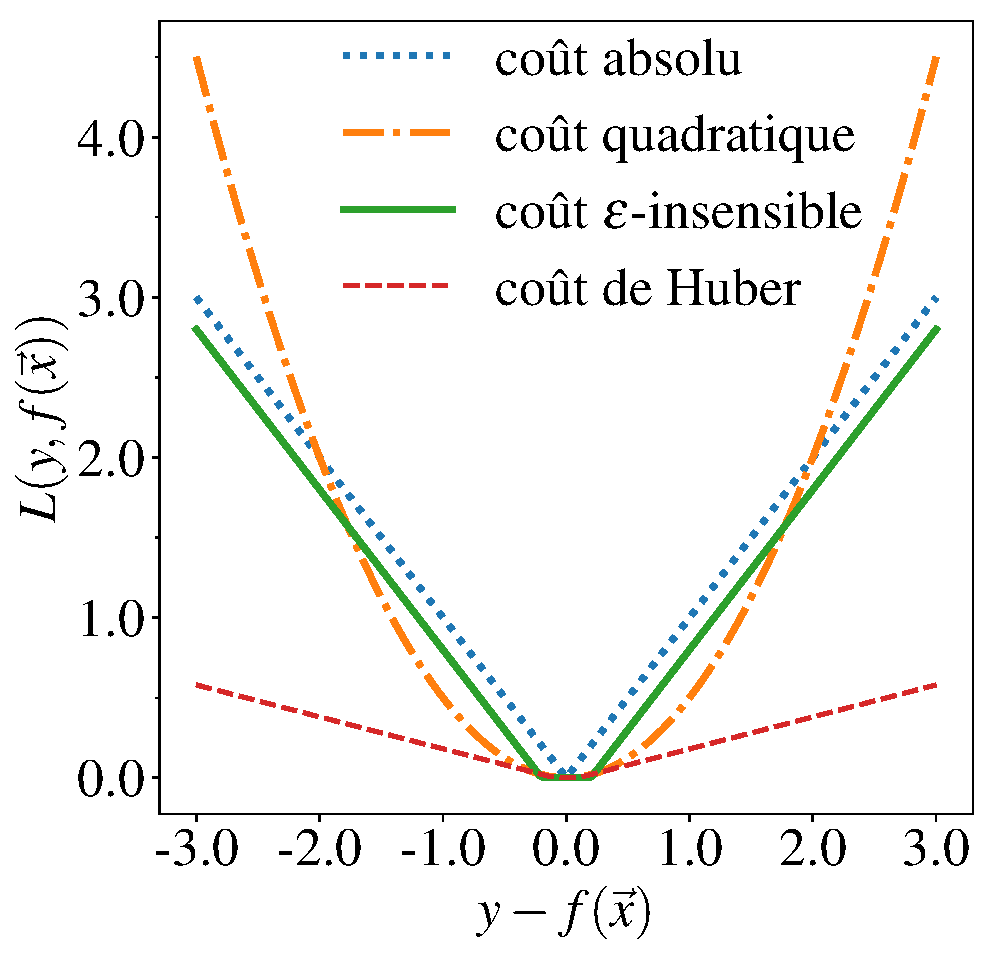
\includegraphics[width=0.5\textwidth]{figures/regression_losses}
%    \end{center}
%  \end{frame}


\documentclass[sans,14pt]{beamer}
\usepackage{pgfpages}
%\setbeameroption{show notes on second screen}
%\setbeameroption{show notes}
\setbeameroption{hide notes}

\usepackage{etex}


\usepackage{fixltx2e} % for \textsubscript


%% Format the bibliography
\usepackage[backend=bibtex,style=alphabetic]{biblatex}
\addbibresource{references}
\setbeamercolor*{bibliography entry title}{fg=MyDarkGrey}
\setbeamercolor*{bibliography entry author}{fg=black}
\setbeamercolor*{bibliography entry location}{fg=black}
\setbeamercolor*{bibliography entry note}{fg=black}
\setbeamertemplate{bibliography item}[text]

% Space between label and reference
\setlength{\biblabelsep}{-15pt}


\mode<presentation>
{
  \usetheme{Copenhagen}
  \usecolortheme{beaver}
  \usefonttheme[onlymath]{serif}
}

%% Change bullet points style
%\setbeamertemplate{itemize items}[triangle]
\setbeamertemplate{itemize items}{{\textemdash}}
\setbeamercolor*{item}{fg=MyDarkGrey}

%% Remove navigation symbols
\setbeamertemplate{navigation symbols}{}
\setbeamertemplate{headline}{}

%% Use only frame number (no total frame count) in footer
\setbeamertemplate{footline}{%
  \raisebox{5pt}{\makebox[\paperwidth]{\hfill\makebox[20pt]{
        \scriptsize\insertframenumber}}}
}

% Adjust margin of itemize environment
\setlength{\leftmargini}{0pt}
\setlength{\leftmarginii}{10pt}
\setlength{\leftmarginiii}{17pt}

%% Adjust font sizes
\setbeamerfont{frametitle}{size=\Large}
\setbeamerfont{normal text}{size=\small}
\setbeamerfont{itemize/enumerate body}{size=\small}
\setbeamerfont{itemize/enumerate subbody}{size=\small}
\setbeamerfont{itemize/enumerate subsubbody}{size=\footnotesize}

%%% To use the Cabin-Condensed fonts
%%% More fonts: see http://www.tug.dk/FontCatalogu
% \usepackage[latin1]{inputenc}
% \usepackage[T1]{fontenc}
% \usepackage[sfdefault]{cabin} 
\usepackage{PTSans} 
\usepackage{PTSansNarrow} 
\renewcommand*\familydefault{\sfdefault} %% Only if the base font of the document is to be sans serif
\usepackage[T1]{fontenc}

\newenvironment{ptnormal}{\fontfamily{PTSans-TLF}\selectfont}{\par}


\usepackage{amsmath}
\usepackage{amsfonts}
\usepackage{amssymb}
\usepackage{amsthm}
\usepackage{bm}
\usepackage{booktabs}
\usepackage{color}
\usepackage{epstopdf}
\usepackage{fancyhdr}
\usepackage{fancybox}
\usepackage[all]{xy}
\usepackage{graphicx}
\usepackage{multirow}
\usepackage[normalem]{ulem}
\usepackage{url}
\usepackage{dsfont}
%


% tikzmark command, for shading over items
\usepackage{tikz}
\usetikzlibrary{calc}
\newcommand{\tikzmark}[1]{\tikz[overlay,remember picture] \node (#1) {};}
\usetikzlibrary{decorations.pathreplacing} % for curly braces
\usepackage[framemethod=tikz]{mdframed} % for fancy title page and other boxes

%% Subfigures
\usepackage[labelformat=simple,caption=false,textfont=scriptsize]{subfig}
\renewcommand{\thesubfigure}{\relax} % do not number captions of
                                     % subfloats


%% to write text at the bottom of a beamer slide
%\def\writeatbottom#1{\vskip 0pt plus 1filll \scriptsize #1}

\newcommand{\topspace}{\rule{0pt}{2.6ex}}
\newcommand{\botspace}{\rule[-1.2ex]{0pt}{0pt}}


%%% Colors
%\usepackage{color}
\definecolor{MyBlue}{rgb}{0.27,0.62,0.73}%{0.,0.2,0.4} 
\definecolor{Aubergine}{rgb}{0.47,0.13,0.44} % 119 33 111
\definecolor{MyTurq}{rgb}{0.,0.8,0.8} 
\definecolor{MyDarkGrey}{rgb}{0.3,0.3,0.3} 
\definecolor{MyMedGrey}{rgb}{0.6,0.6,0.6} 
\definecolor{MyLightGrey}{rgb}{0.95,0.95,0.95} 
\definecolor{MyDarkRed}{rgb}{0.8,0.,0.} 
\definecolor{MyOrange}{rgb}{0.93,0.56,0.25}
\definecolor{MyPink}{rgb}{0.73,0.27,0.39}
\definecolor{MyLightYellow}{HTML}{FFFFCC}
%\usepackage[colorlinks=true,citecolor=MyTurq]{hyperref}
\AtEveryCite{\color{MyMedGrey}}

\newcommand{\blue}[1]{{\color{MyBlue}{\textbf{#1}}}}
\newcommand{\red}[1]{{\color{MyOrange}{\textbf{#1}}}}
\newcommand{\black}[1]{{\color{MyDarkGrey}{\textbf{#1}}}}
\newcommand{\yellow}[1]{{\color{MyLightYellow}{\textbf{#1}}}}

\newcommand{\TODO}{{\color{MyDarkRed}{TODO~}}}

\setbeamercolor{normal text}{fg=MyDarkGrey}
\setbeamercolor{frametitle}{fg=Aubergine}

%%% ---- Titre des slides  (underline) ----------------
\setbeamertemplate{frametitle}{%
    \usebeamerfont{frametitle}\insertframetitle\strut%
    \vskip-.05\baselineskip%
    \leaders\vrule width \paperwidth\vskip1.pt%
    \vskip0pt%
    \nointerlineskip
}
%%% ---------------------------------------------------


% --- Math symbols -------------------------------------------------------------
\newcommand{\EE}{{\mathbb E}}
\newcommand{\PP}{{\mathbb P}}
\newcommand{\NN}{{\mathbb N}}
\newcommand{\RR}{{\mathbb R}}

\newcommand{\avec}{\vec{a}}
\newcommand{\alphavec}{\vec{\alpha}}
\newcommand{\betavec}{\vec{\beta}}
\newcommand{\cvec}{\vec{c}}
\newcommand{\fvec}{\vec{f}}
\newcommand{\muvec}{\vec{\mu}}
\newcommand{\mvec}{\vec{m}}
\newcommand{\rvec}{\vec{r}}
\newcommand{\thetavec}{\vec{\theta}}
\newcommand{\xvec}{\vec{x}}
\newcommand{\yvec}{\vec{y}}
\newcommand{\wvec}{\vec{w}}
\newcommand{\uvec}{\vec{u}}
\newcommand{\vvec}{\vec{v}}
\newcommand{\zvec}{\vec{z}}

% \newcommand{\amat}{{\mathbf A}}}
% \newcommand{\dmat}{{\mathbf D}}
% \newcommand{\gmat}{{\mathbf G}}
% \newcommand{\kmat}{{\mathbf K}}
% \newcommand{\lmat}{{\mathbf L}}
% \newcommand{\mmat}{{\mathbf M}}
% \newcommand{\wmat}{{\mathbf W}}
% \newcommand{\xmat}{{\mathbf X}}

\newcommand{\aset}{\mathcal{A}}
\newcommand{\cset}{\mathcal{C}}
\newcommand{\dset}{\mathcal{D}}
\newcommand{\fcal}{\mathcal{F}}
\newcommand{\hcal}{\mathcal{H}}
\newcommand{\ncal}{\mathcal{N}}
\newcommand{\nset}{\mathcal{N}}
\newcommand{\rcal}{\mathcal{R}}
\newcommand{\sset}{\mathcal{S}}
\newcommand{\vset}{\mathcal{V}}
\newcommand{\tset}{\mathcal{T}}
\newcommand{\xcal}{\mathcal{X}}
\newcommand{\ycal}{\mathcal{Y}}

\newcommand{\lzeronorm}[1]{\left|\left|#1\right|\right|_0}
\newcommand{\lonenorm}[1]{\left|\left|#1\right|\right|_1}
\newcommand{\ltwonorm}[1]{\left|\left|#1\right|\right|_2}

\usepackage{bbm}
\newcommand{\indic}{\mathbbm{1}}

\DeclareMathOperator*{\argmin}{arg\,min}
\DeclareMathOperator*{\argmax}{arg\,max}
\graphicspath{{./figures/}}

% ------------------------------------------------------------------------------



% \newcommand{\source}[1]{\begin{textblock*}{4cm}(8.7cm,8.6cm)
%     \begin{beamercolorbox}[ht=0.5cm,right]{framesource}
%       \usebeamerfont{framesource}\usebeamercolor[fg]{framesource} Credits: {#1}
%     \end{beamercolorbox}
% \end{textblock*}}




\newcommand{\mytitle}{Fondamentaux du Machine Learning}
\author[Walter]{Thomas Walter \and  Chlo\'e-Agathe~Azencott \and Florian Massip} 
\institute[CBIO]{\inst{1} Centre for Computational Biology(CBIO), Mines Paris, PSL University\and %
                      \inst{2} Institut Curie\and
                      \inst{3} U1331 - INSERM}

\date{\small \today}

\begin{document}
{

  \begin{frame}[plain]
    \fontfamily{PTSansNarrow-TLF}\selectfont
    \begin{center}
      {\ptnormal{\textit{Formation Chef de Projet IA}}}
    \end{center}

    \vspace{70pt}

    \centerline{{\Large \bf \mytitle}}

    \vspace{15pt}

    \centerline{\insertauthor}

    \vspace{15pt}

    {\footnotesize
      \centerline{Center for Computational Biology (CBIO)}
    
      \centerline{Mines Paris -- Institut Curie -- INSERM U900}

      \centerline{PSL Research University \& PR[AI]RIE, Paris, France}
    }

    \centerline {\insertdate}

\end{frame}

% Do not count title slide when numbering frames
\addtocounter{framenumber}{-1}


% Overview
\begin{frame}
  \frametitle{Programme}

  \begin{itemize}
  \item Introduction à l'apprentissage automatique
  \item \blue{Cours 1 :} Minimisation du risque empirique 
  \item \blue{Cours 2 :} Régularisation et sélection de modèle
  \item \blue{Cours 3 :} Arbres et méthodes ensemblistes
  \item \blue{Cours 4 :} Méthodes à noyaux 
  \item \blue{Cours 5 :} Réduction de dimension
  \item \blue{Cours 6 :} Clustering
  \item Travaux pratiques : mise en œuvre des notions et algorithmes avec scikit-learn (Python numérique).
\end{itemize}
\end{frame}





\begin{frame}
  \begin{center}
    \red{\LARGE Cours 6 -- Clustering} 
  \end{center}
\end{frame}

\begin{frame}
  \frametitle{Clustering ou partitionnement}
  \begin{itemize}
  \item \red{Clustering :} partitionner les données en sous-ensembles (\red{clusters}) homogènes
  \item Exemples :
    \begin{itemize}
    \item \blue{segmentation de marché}
    \item \blue{communautés} sur un réseau social
    \item \blue{topic modeling} (thématique de textes)
    \item \blue{compression} ou \blue{segmentation d'images}
    \item \blue{sous-types} d'une maladie
  \end{itemize}
  \end{itemize}
\end{frame}

\begin{frame}
  \frametitle{Clustering : Motivation}
  \begin{itemize}
  \item Étude de données \blue{non-étiquetées}
  \item Analyse \blue{exploratoire}
  \item \blue{Visualisation}
  \item Peut précéder une phase d'\blue{inférence} (ex. topic modeling)
  \end{itemize}
\end{frame}


\begin{frame}
  \begin{center}
    \large{1. Évaluation d'un clustering}
  \end{center}
\end{frame}

\begin{frame}
  \frametitle{1.1 Critères géométriques}
  \begin{center}
    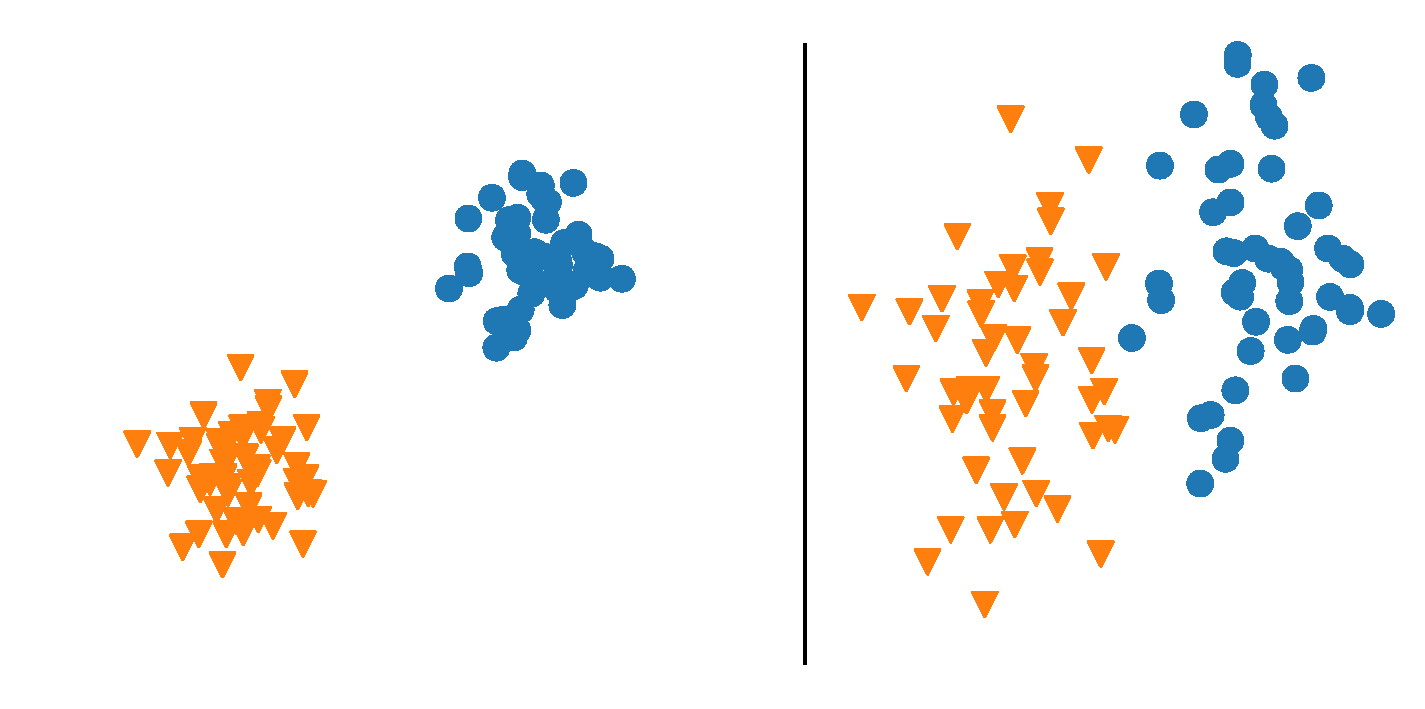
\includegraphics[width=0.5\textwidth]{figures/homogeneity}%
  \end{center}
  \begin{minipage}[t]{0.5\linewidth}
    \begin{itemize}
    \item \red{Homogénéité} \textcolor{gray!70}{(tightness)}
      \begin{itemize}
      \item Pour le cluster $k$ :
        \begin{equation*}
          T_k = \frac{1}{|\cset_k|} \sum_{\xvec \in \cset_k} d(\xvec, \muvec_k)
        \end{equation*}
      \end{itemize}
    \end{itemize}
  \end{minipage}%
  \begin{minipage}[t]{0.5\linewidth}
    \begin{itemize}
    \item \red{Centroïde} du cluster $\cset$:
      \[ \muvec_{\cset} = \frac{1}{\cset}\sum_{\xvec \in \cset}\xvec\]
    \item \red{Médoïde} : l'élément de $\cset$ le plus proche de $\muvec_{\cset}$
    \end{itemize}  
  \end{minipage}
  \begin{itemize}
  \item[]  
    \begin{itemize}
    \item Pour le clustering complet :  $T = \frac1K\sum_{k=1}^{K}T_k$
    \end{itemize}
  \end{itemize}
\end{frame}

\begin{frame}
  \frametitle{1.1 Critères géométriques}
  \begin{center}
    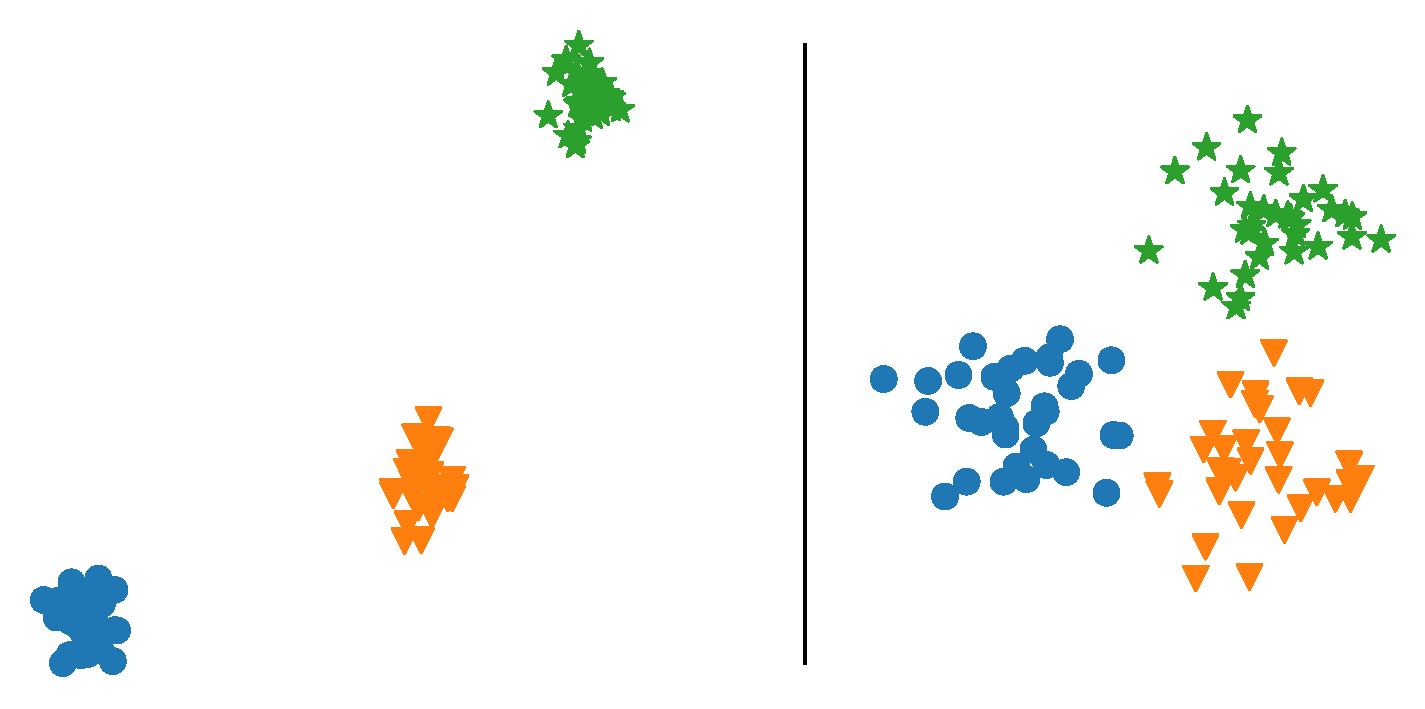
\includegraphics[width=0.5\textwidth]{figures/separability}%
  \end{center}
  \begin{itemize}
  \item \red{Séparabilité}
    \begin{itemize}
    \item Pour les clusters $k$ et $l$ : 
      \begin{equation*}
        s_{kl} = d(\muvec_k, \muvec_l)
      \end{equation*}
    \item Pour le clustering :
      \begin{equation*}
	S = \frac{2}{K(K-1)}\sum_{k=1}^{K-1}\sum_{l=k+1}^{K}s_{kl}
      \end{equation*}
    \end{itemize}
  \end{itemize}
\end{frame}

\begin{frame}
  \frametitle{1.1 Critères géométriques}
  \begin{itemize}
  \item \red{Coefficient de silhouette}
    \begin{itemize}
    \item Pour un point $\xvec$ :
      {\footnotesize
      \begin{align*}
	a(\xvec) & = \frac{1}{|\cset_{k(\xvec)}| - 1} \sum_{\uvec \in \cset_{k(\xvec)}}d(\xvec, \uvec) \\
	b(\xvec) & = \min_{l\neq k(\xvec)}\frac{1}{|\cset_l|} \sum_{u \in \cset_l}d(\uvec, \xvec) \\
        s(\xvec) & = \frac{b(\xvec) - a(\xvec)}{\max(a(\xvec), b(\xvec))}
      \end{align*}}

  \item Pour le clustering :
      \begin{equation*}
        s = \frac1n \sum_{i=1}^n s(\xvec^i).
      \end{equation*}
    \end{itemize}
  \end{itemize}
\end{frame}

\begin{frame}
  \frametitle{1.2 Stabilité des clusters}
    \begin{center}
      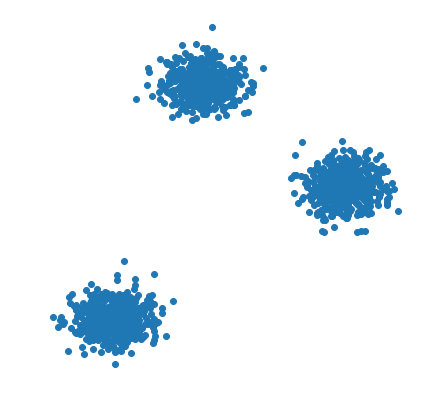
\includegraphics[width=0.7\textwidth]{figures/three_clusters}%
    \end{center}
\end{frame}

\begin{frame}
  \frametitle{1.3 Comparaison à des étiquettes connues}
  \begin{itemize}
  \item Difficulté : les clusters sont numérotés arbitrairement
  \item \red{Indice de Rand}
        \begin{equation*}
      \text{RI} = \frac2{n (n-1)} \sum_{i=1}^n \sum_{l=i+1}^n 
      \indic_{k(\xvec^i) = k(\xvec^l)} \, \indic_{y^i = y^l} + 
      \indic_{k(\xvec^i) \neq k(\xvec^l)} \, \indic_{y^i \neq y^l}.
    \end{equation*}
  \end{itemize}
\end{frame}

\begin{frame}
  \begin{center}
    \large{2. Clustering hiérarchique}
  \end{center}
\end{frame}

\begin{frame}
  \frametitle{Dendrogramme}
  \begin{center}
    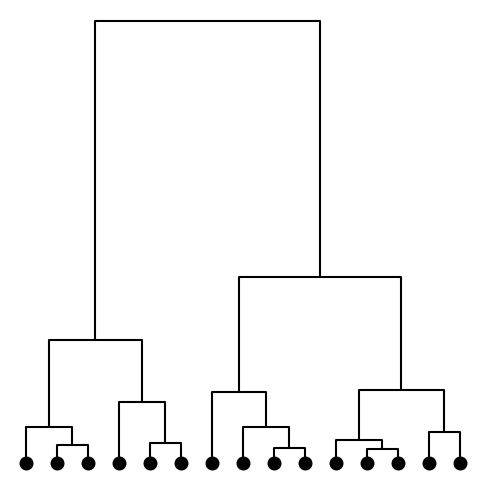
\includegraphics[width=0.7\textwidth]{figures/dendrogram}%
  \end{center}
\end{frame} 

\begin{frame}
  \frametitle{Construction}
  \begin{itemize}
  \item Construction \red{agglomérative} \textcolor{gray!70}{(bottom-up)}
    \begin{itemize}
    \item Initialement : chaque point est son propre cluster 
    \item On fusionne itérativement les clusters les plus proches
    \end{itemize}
  \item Construction \red{divisive} \textcolor{gray!70}{(top-down)}
    \begin{itemize}
    \item Intialement : tous les points sont dans le même cluster 
    \item On sépare itérativement les clusters en deux
    \end{itemize}
  \end{itemize}
\end{frame}

\begin{frame}
  \frametitle{Fonctions de lien}
  \begin{itemize}
  \item \red{Fonction de lien} \textcolor{gray!70}{(linkage)} : distance entre deux clusters
    \begin{itemize}
    \item \red{Lien simple} \textcolor{gray!70}{(single linkage)}
      \[ d_{\text{simple}}(\cset_k, \cset_l) = \min_{(\uvec, \vvec) \in \cset_k \times \cset_l } d(\uvec, \vvec).
      \]
      \pause
    \item \red{Lien complet} \textcolor{gray!70}{(complete linkage)}
      \[
        d_{\text{complet}}(\cset_k, \cset_l) = \max_{(\uvec, \vvec) \in \cset_k \times \cset_l} d(\uvec, \vvec).
      \]
      \pause
    \item \red{Lien moyen} \textcolor{gray!70}{(average linkage)} ou UPGMA \textcolor{gray!70}{(Unweighted Paired Group Method with Arithmetic mean)}
      \[
        d_{\text{moyen}}(\cset_k, \cset_l) = \frac1{\lvert \cset_k \rvert} 
        \frac1{\lvert \cset_l \rvert}
        \sum_{\uvec \in \cset_k}\sum_{\vvec \in \cset_l} d(\uvec, \vvec).
      \]
    \end{itemize}
  \end{itemize}
\end{frame}

\begin{frame}[t]
  \frametitle{Fonctions de lien}
  \begin{itemize}
  \item \red{Fonction de lien} \textcolor{gray!70}{(linkage)} : distance entre deux clusters
    \begin{itemize}
    \item \red{Lien centroïdal} \textcolor{gray!70}{(centroid linkage)}
      \[
        d_{\text{centroidal}}(\cset_k, \cset_l) = d \left (\frac1{\lvert \cset_k \rvert} 
          \sum_{\uvec \in \cset_k} \uvec, 
          \frac1{\lvert \cset_l \rvert} \sum_{\vvec \in \cset_l} \vvec \right) = 
        d(\muvec_k, \muvec_l).
      \]
    \end{itemize}
  \end{itemize}
\end{frame}


\begin{frame}
  \begin{center}
    \large{3. Algorithme des k-moyennes}
  \end{center}
\end{frame}

\begin{frame}
  \frametitle{Variance intra-cluster}
  \begin{itemize}
  \item \red{Variance intra-cluster}
    \[
            \text{Var}_\text{in}(\cset) = \frac1{\lvert \cset \rvert} \sum_{\xvec \in \cset}
      \ltwonorm{\xvec - \muvec}^2.
    \]
  \item Minimiser la variance intra-cluster : créer des clusters \blue{homogènes}
  \end{itemize}
\end{frame}

\begin{frame}
  \frametitle{Algorithme de Lloyd}
  \begin{itemize}
  \item \blue{Initialisation :} choisir les $\muvec_1, \muvec_2, \ldots, \muvec_K$ parmi les données. 
  \item \blue{Affecter} chaque observation $\xvec \in \dset$ au centroïde dont elle est le plus proche :
    \begin{equation*}
      k(\xvec^i) = \argmin_{k=1, \ldots, K}\ltwonorm{\xvec^i - \muvec_k}^2
    \end{equation*}
  \item \blue{Recalculer} les centroïdes $\muvec_k$. 
  \item \blue{Répéter} jusqu'à ce que les affectations ne changent plus. 
  \end{itemize}
\end{frame}

\begin{frame}
  \frametitle{Algorithme de Lloyd}
  \begin{itemize}
  \item \blue{Avantages :}
    \begin{itemize}
    \item Converge rapidement en pratique
    \end{itemize}
    \pause
  \item \blue{Inconvénients :}
    \begin{itemize}
    \item Nécessité de fixer $K$ 
    \item Approche \blue{gloutonne} : pas de garantie de minimum global
    \item \blue{Stochasticité} : dépend de l'initialisation \pause $\rightarrow$ k-means++ 
    \item Clusters nécessairement \blue{convexes} \pause $\rightarrow$ kernel k-means
    \end{itemize}
  \end{itemize}
\end{frame}

\begin{frame}
  \begin{center}
    \large{4. DBSCAN}
  \end{center}
\end{frame}

\begin{frame}
  \frametitle{DBSCAN: Motivation}
  \begin{center}
    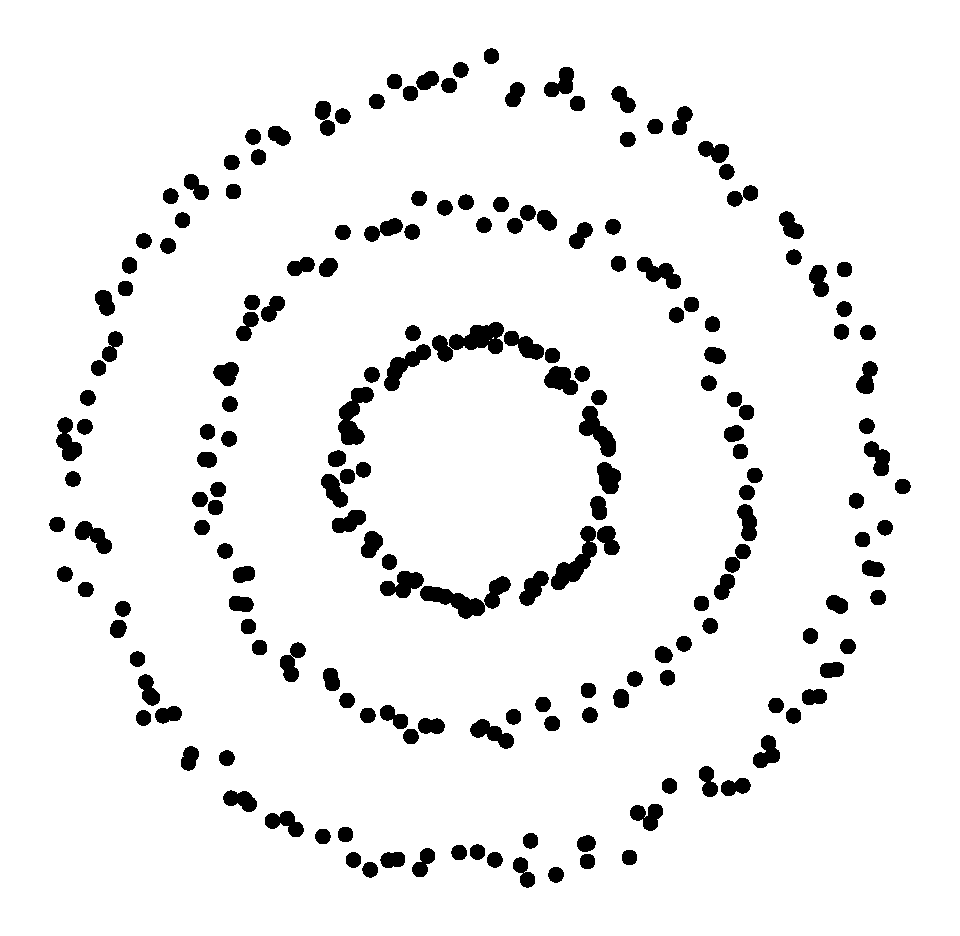
\includegraphics[width=.3\textwidth]{figures/dbscan_pb}%
    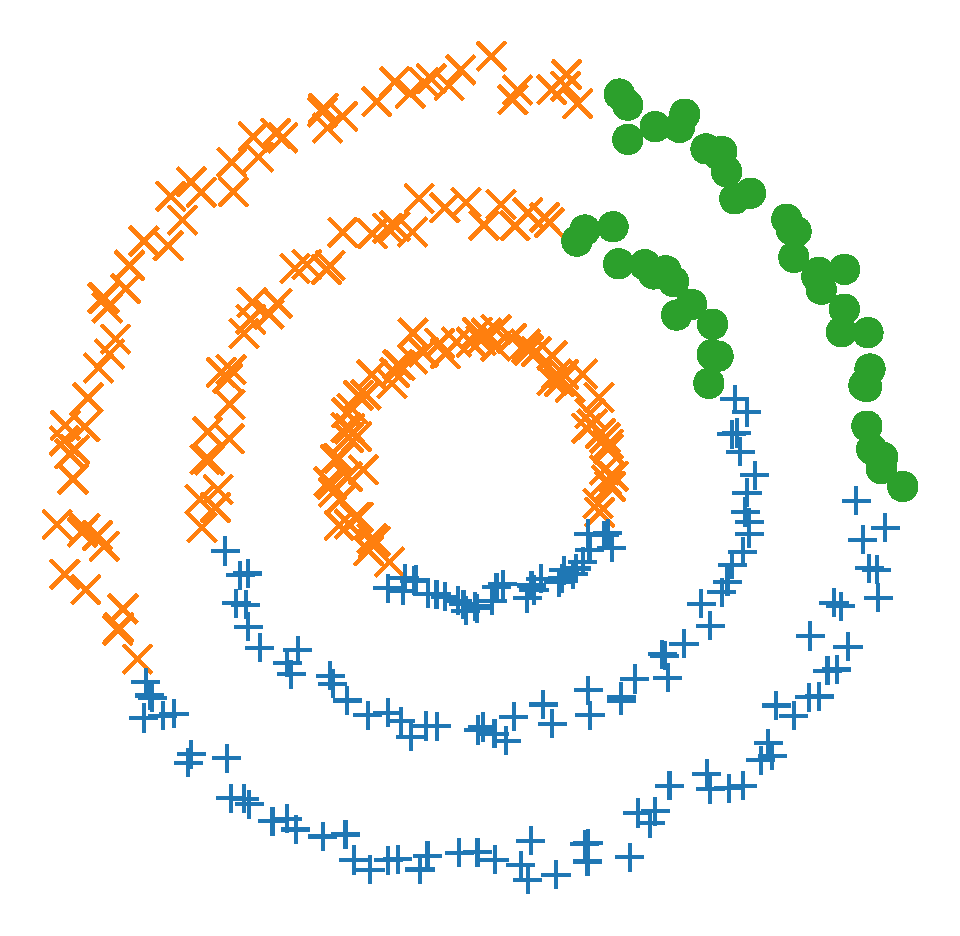
\includegraphics[width=.3\textwidth]{figures/hierarchical_sol}%
    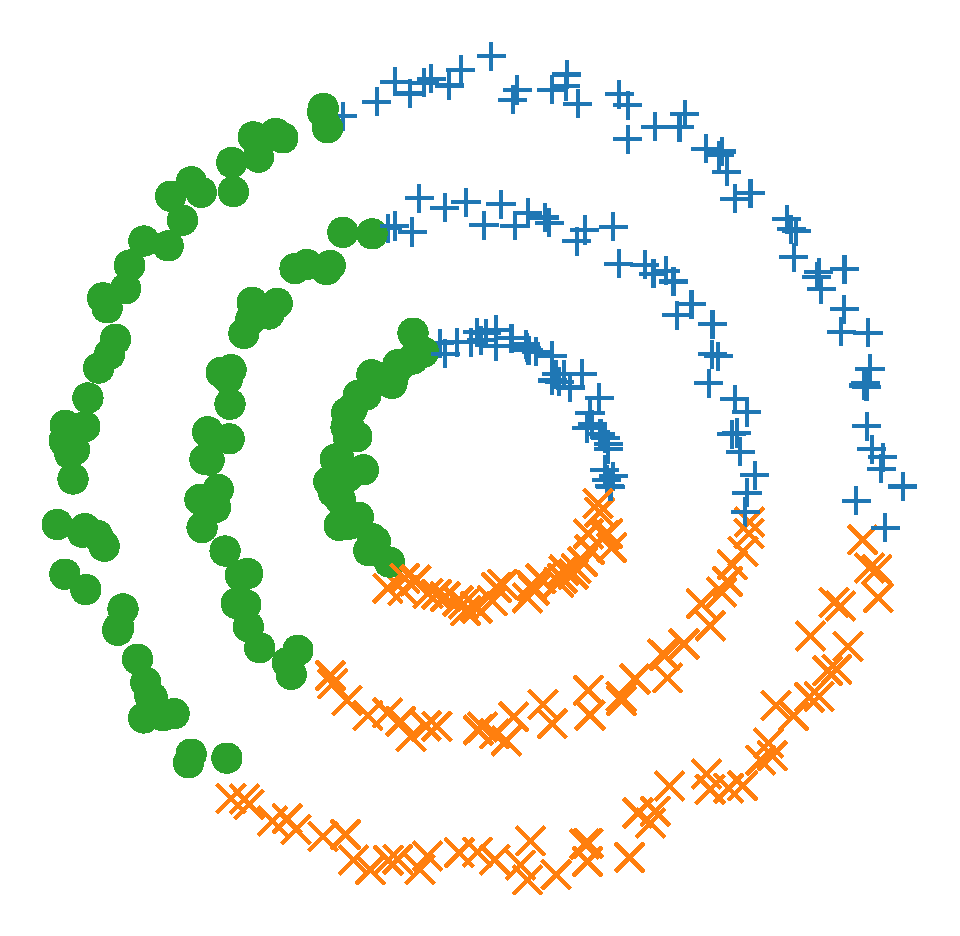
\includegraphics[width=.3\textwidth]{figures/kmeans_sol}
  \end{center}
  \begin{itemize}
  \item Idée : utiliser la \blue{densité}
  \end{itemize}
\end{frame}


\begin{frame}
  \frametitle{DBSCAN}
  \begin{itemize}
  \item Idée : itérer \blue{de proche en proche} par des \blue{voisinages} (boules) de rayon $\epsilon$
  \item Les points \blue{isolés} (min $n_{\min}$ points par cluster) sont du bruit 
  \end{itemize}
  \begin{center}
    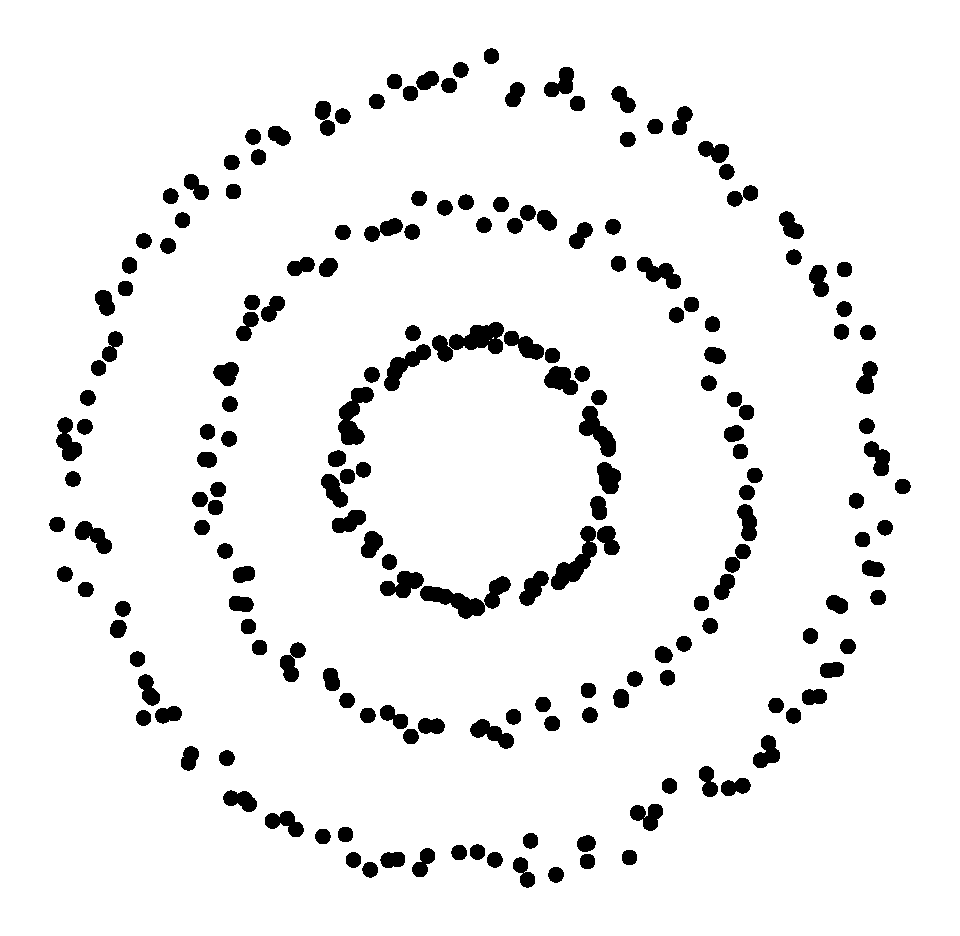
\includegraphics[width=.6\textwidth]{figures/dbscan_pb}
  \end{center}
\end{frame}

\begin{frame}
  \frametitle{DBSCAN : avantages et inconvénients}
  \begin{itemize}
  \item \blue{Avantages :}
    \begin{itemize}
    \item n'impose pas de forme particulière
    \item simple, pas de définition du nombre de clusters
    \item robustesse aux données aberrantes
    \end{itemize}
  \pause
  \item \blue{Inconvénients :}
    \begin{itemize}
    \item ne sait pas gérer des écarts
    \item peu de résultats théoriques
    \item pas applicable en très haute dimension 
    \end{itemize}
  \end{itemize}
\end{frame}


\begin{frame}
  \frametitle{Recap}
\end{frame}


\end{document}
